\documentclass[11pt,letterpape, fleqn]{article}
\usepackage[lmargin=1in,rmargin=1in,tmargin=1in,bmargin=1in]{geometry}

% -------------------
% Packages
% -------------------
\usepackage{
	amsmath,			% Math Environments
	amssymb,			% Extended Symbols
	enumerate,		% Enumerate Environments
	graphicx,			% Include Images    
	lastpage,			% Reference Lastpage
	multicol,			% Use Multi-columns
	multirow,			% Use Multi-rows
	siunitx
}

\graphicspath{{./images/}}

\usepackage{wrapfig}

% -------------------
% Font
% -------------------
\usepackage[T1]{fontenc}
\usepackage{charter}    


% -------------------
% Heading Commands
% -------------------
\newcommand{\class}{Mu Alpha Theta}
\newcommand{\term}{2022-2023}
\newcommand{\head}[4]{%
\thispagestyle{empty}
\vspace*{-0.5in}
\noindent\begin{tabular*}{\textwidth}{l @{\extracolsep{\fill}} r @{\extracolsep{6pt}} l}
	\textbf{#1} & \textbf{Name:} & \makebox[5.75cm]{\hrulefill} \\
	\textbf{#2} & & \\
	\textbf{\class:\; \term} & & \\
\end{tabular*} \\
\rule[2ex]{\textwidth}{2pt} %
}


% -------------------
% Commands
% -------------------
\newcommand{\prob}{\noindent\textbf{Problem. }}
\newcounter{problem}
\newcommand{\problem}{
	\stepcounter{problem}%
	\noindent \textbf{Problem \theproblem. }%
}
\newcommand{\pointproblem}[1]{
	\stepcounter{problem}%
	\noindent \textbf{Problem \theproblem.} (#1 points)\,%
}
\newcommand{\pspace}{\par\vspace{\baselineskip}}
\newcommand{\ds}{\displaystyle}


% -------------------
% Header & Footer
% -------------------
\usepackage{fancyhdr}

\fancypagestyle{pages}{
	%Headers
	\fancyhead[L]{}
	\fancyhead[C]{}
	\fancyhead[R]{}
\renewcommand{\headrulewidth}{0pt}
	%Footers
	\fancyfoot[L]{}
	\fancyfoot[C]{}
	\fancyfoot[R]{}
\renewcommand{\footrulewidth}{0.0pt}
}
\headheight=0pt
\footskip=14pt

\pagestyle{pages}


% -------------------
% Content
% -------------------

\begin{document}
\head{Worksheet \#6}{Date:}
\centering

% Question 1: 20201 (2000 AMC10)
\begin{minipage}{\textwidth}
	\problem

	\begin{wrapfigure}[11]{r}{0.6\textwidth}
		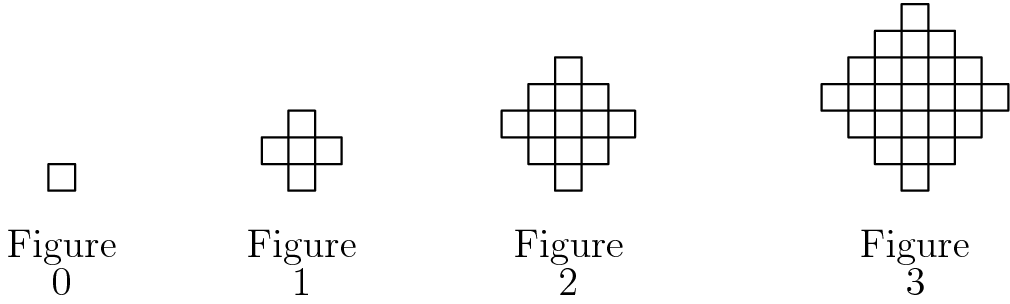
\includegraphics[width = 10cm]{images:q8.png}
   \end{wrapfigure}
   \noindent Figures $0$, $1$, $2$, and $3$ consist of $1$, $5$, $13$, and $25$ nonoverlapping unit squares, respectively. If the pattern were continued, how many nonoverlapping unit squares would there be in figure $100$?

    \vspace{7cm}
\end{minipage}

% Question 2: Thursday (2000 AMC10)
\begin{minipage}{\textwidth}
    \problem

   \noindent In year $N$, the $300^{\text{th}}$ day of the year is a Tuesday. In year $N+1$, the $200^{\text{th}}$ day is also a Tuesday. On what day of the week did the $100$th day of year $N-1$ occur?
	
   \vspace{4cm}
\end{minipage}

% Question 3: 2pi = 2.28 (2002 AMC10A)

\begin{minipage}{\textwidth}
    \problem

	\begin{wrapfigure}[11]{r}{0.3\textwidth}
		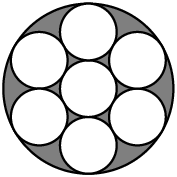
\includegraphics[width = 4cm]{images:q5.png}
   \end{wrapfigure}
   \noindent Each of the small circles in the figure has radius one. The innermost circle is tangent to the six circles that surround it, and each of those circles is tangent to the large circle and to its small-circle neighbors. Find the area of the shaded region.

   \vspace{4cm}
\end{minipage}

% Question 4: 1/(1+sin(theta)) (2000 AMC12)
\begin{minipage}{\textwidth}
    \problem

	\begin{wrapfigure}[11]{r}{0.3\textwidth}
		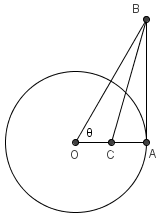
\includegraphics[width = 4cm]{images-q7.png}
   \end{wrapfigure}
   \noindent A circle centered at $O$ has radius $1$ and contains the point $A$. The segment $AB$ is tangent to the circle at $A$ and $\angle AOB = \theta$. If point $C$ lies on $\overline{OA}$ and $\overline{BC}$ bisects $\angle ABO$, then $OC =$

   \vspace{7cm}
\end{minipage}

% Question 5: 1680 (2000 AMC12)

\begin{minipage}{\textwidth}
    \problem

	\begin{wrapfigure}[11]{l}{0.5\textwidth}
		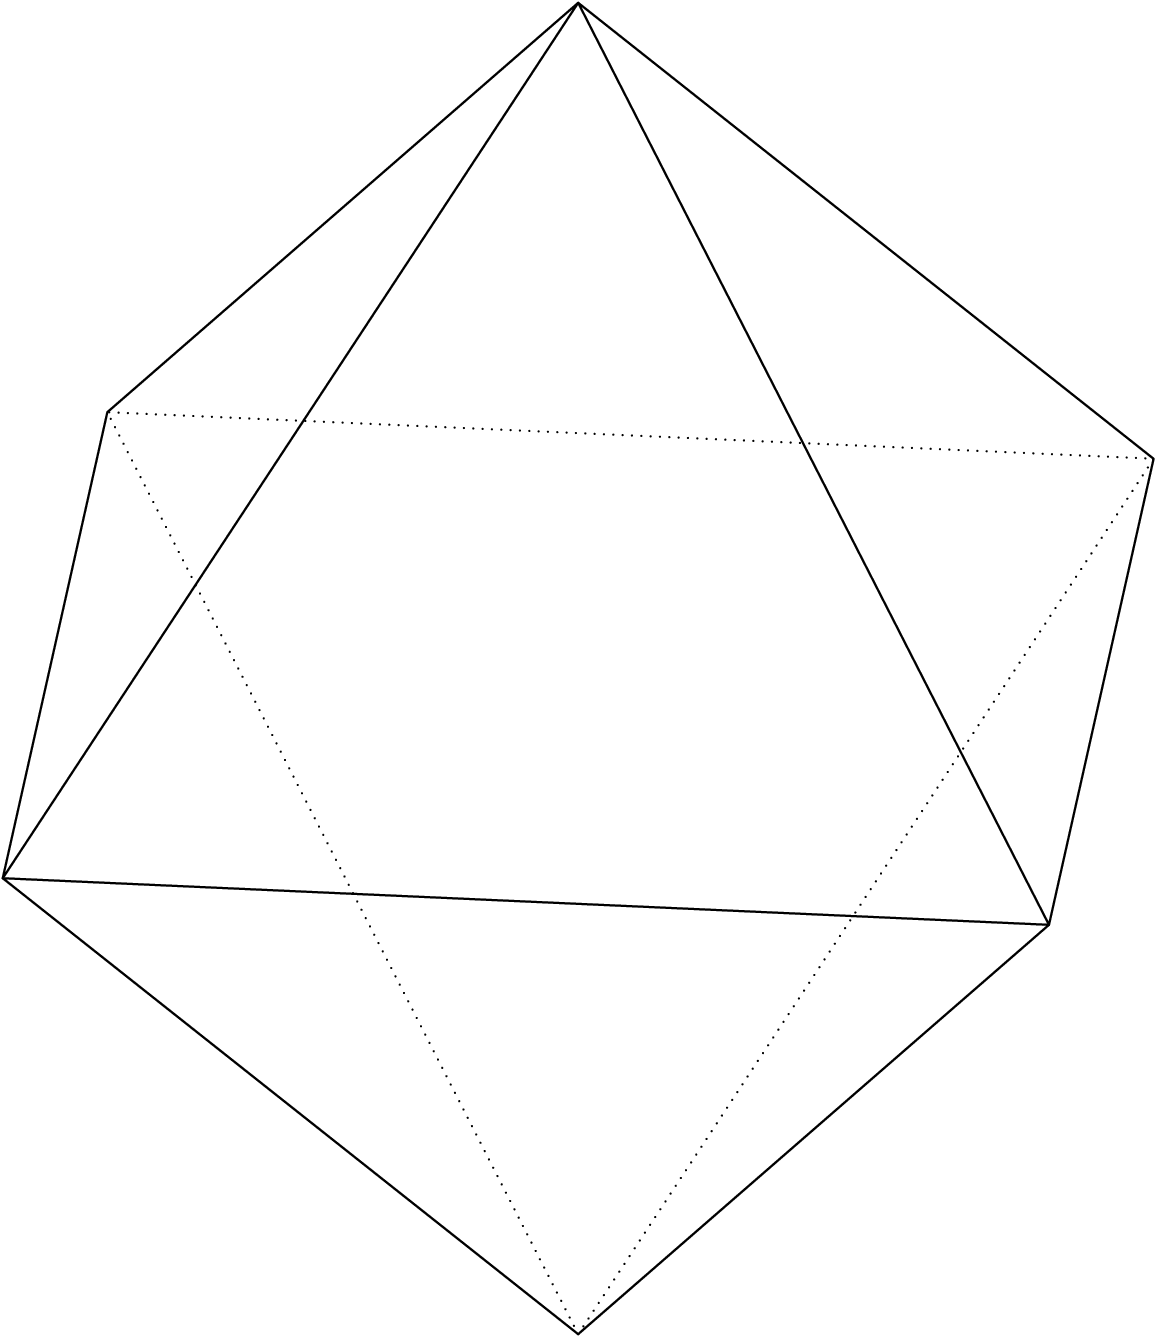
\includegraphics[width = 7cm]{images-q25.png}
   \end{wrapfigure}
   \noindent Eight congruent equilateral triangles, each of a different color, are used to construct a regular octahedron. How many distinguishable ways are there to construct the octahedron? (Two colored octahedrons are distinguishable if neither can be rotated to look just like the other.)

   \vspace{8cm}
\end{minipage}

\vspace{6cm}
\end{document}
